\chapter{PENDAHULUAN} \label{ch:chapter_1}

\section{Latar Belakang}
Badan Pusat Statistik (BPS) merupakan suatu lembaga pemerintah non-departemen yang bertanggung jawab dalam penyediaan statistik dasar \cite{_badan_????}. Dalam peranannya sebagai penyedia data, BPS melakukan pengumpulan data dengan 2 (dua) metode : primer dan sekunder. Pengumpulan data primer berarti BPS secara mandiri mengumpulkan data dengan menggunakan metode wawancara langsung dengan responden, baik responden individu, rumah tangga, maupun perusahaan. Sementara pengumpulan data sekunder berarti BPS memperoleh data dari pihak lain.

Dalam melakukan kegiatan perstatistikan, yang selanjutnya merujuk kepada pengumpulan data primer, BPS merujuk kepada \textit{General Statistical Business Process Model} (GSBPM) ~\cite{_gsbpm_????}. GSBPM merupakan suatu standard arsitektur bisnis kegiatan perstatistikan yang dirumuskan oleh \textit{United Nations Economic Commission for Europe} (UNECE). Dalam GSBPM, \textit{Business Process} Statistik dibagi menjadi 8 (tujuh) phase : \textit{Specify Needs}, \textit{Design}, \textit{Build}, \textit{Collect}, \textit{Process}, \textit{Analyze}, \textit{Disseminate}, dan \textit{Evaluate}, dimana masing-masing phase dapat dijabarkan lagi dalam beberapa sub-proses.

\begin{figure}
    \centering
    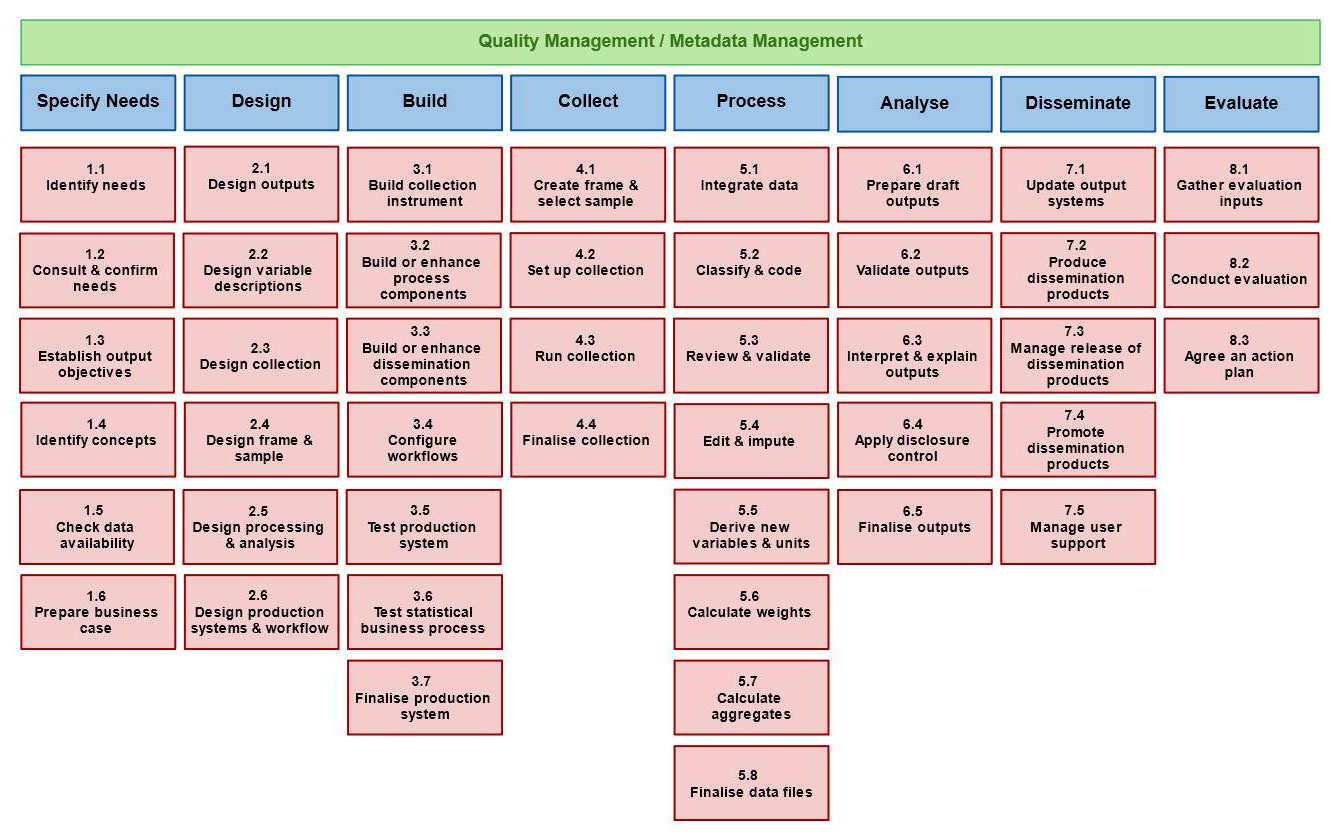
\includegraphics[width=13cm]{../../Resources/Images/gsbpm}
    \caption{\textit{Statistical Business Process Phases} dalam GSBPM}
    \label{fig:gsbpm}
\end{figure}

Pengumpulan dan pengolahan data dalam GSBPM tercakup dalam 3 (tiga) fase, yaitu : \textit{Collect Phase}, \textit{Process Phase}, dan \textit{Analyze Phase}. \textit{Collect phase} adalah fase dimana semua informasi (data dan metadata) dikumpulkan dengan menggunakan beberapa metode pengumpulan (termasuk ekstraksi dari register dan database statistik, administratif, maupun yang lain), dan memuatkannya ke dalam suatu \textit{environment} untuk pemrosesan lebih lanjut. \textit{Process phase} adalah fase dimana data dibersihkan dan dipersiapkan untuk tahap berikutnya, yaitu \textit{analysis phase}. \textit{Collect phase} dan \textit{process phase} dapat dilakukan secara berulang dan paralel. Fase terakhir sebelum data siap untuk didesiminasikan adalah \textit{analyze phase}. Pada tahap \textit{analyze phase}, data ditransformasikan kedalam bentuk \textit{statistical output} yang disesuaikan dengan kebutuhan (\textit{fit for purpose}).

Kondisi saat ini, \textit{process phase} dan \textit{analyze phase} merupakan tahapan yang memiliki ketergantungan akan Teknologi Informasi dan Komunikasi (TIK) yang sangat besar. \textit{Process phase} merupakan tahapan dimana dilakukan input data hasil pendataan lapangan dari format kuesioner ke dalam format digital, termasuk didalamnya pengkodean, imputasi, validasi, dan penghitungan penimbang. Sementara \textit{analyze phase} memerlukan keterlibatan software analisis yang membantu mentransformasikan data menjadi sebuah informasi. Adapun \textit{collect phase}, meskipun saat ini masih menggunakan pengumpulan data dengan mengadopsi \textit{paper questionaire}, tetapi kedepannya akan dilakukan transformasi dengan menggunakan metode \textit{Computer Assisted Personal Interviewing} (CAPI)\footnote{Keterangan Dr. Said Mirza Pahlevi, M.Eng., Kepala Subdirektorat Pengembangan Basis Data, 24 Februari 2016}, meskipun feasibility-nya belum pernah diujicobakan\footnote{Keterangan Dr. Muchammad Romzi, Kepala Subdirektorat Pengembangan Model Statistik, 4 Maret 2016}. 

Penggunaan metode CAPI dalam pengumpulan data yang dilakukan BPS, sedikit banyak akan mengubah paradigma pengumpulan dan pengolahan data yang selama ini telah berjalan. Pengumpulan dan pengolahan data selama ini merupakan dua buah tahapan yang terpisah. Dengan diterapkannya CAPI maka beberapa sub-proses dari \textit{process phase}, seperti pengkodean dan validasi, dapat dilakukan secara terintegrasi dengan pengumpulan data. Penggunaan CAPI (\textit{device}) juga dapat menghemat waktu dan biaya \cite{wright_researching_2005}. Metode CAPI sebenarnya bukanlah sebuah hal yang baru. Metode ini sudah ada sejak beberapa dekade terakhir ~\cite{_redesigning_????}. Bahkan sebuah penelitian yang dilakukan oleh Gary Klein dkk menyatakan pengumpulan data dengan menggunakan metode CAPI berpotensi terjadi bias, terutama dalam akurasi, \textit{completeness}, dan \textit{item omission} ~\cite{klein_bias_1996}. Akan tetapi, dengan semakin berkembangnya teknologi \textit{mobile computing} yang dipadukan dengan penggunaan \textit{Web service} ~\cite{tergujeff_mobile_2007}, maka potensi bias dapat dikurangi dengan merancang sejumlah \textit{service} yang berfungsi untuk menvalidasi hasil pendataan.

Implementasi \textit{Web service} pada pengumpulan data dengan menggunakan CAPI bukanlah tanpa kendala. Petugas pengumpulan data harus berpindah-pindah dari satu lokasi pendataan ke lokasi yang lain untuk mengunjungi responden. Dikarenakan keterbatasan infrastruktur seperti sinyal telekomunikasi dan daya tahan baterai dari \textit{device} yang digunakan, seringkali tidak mudah bagi \textit{device} untuk selalu terhubung dengan jaringan internet dan berkomunikasi dengan \textit{Web service}. \textit{Device} setiap saat dapat dengan mudah berubah dari \textit{connected node} menjadi \textit{disconnected node} dan sebaliknya. 

\begin{figure}[h]
    \centering
    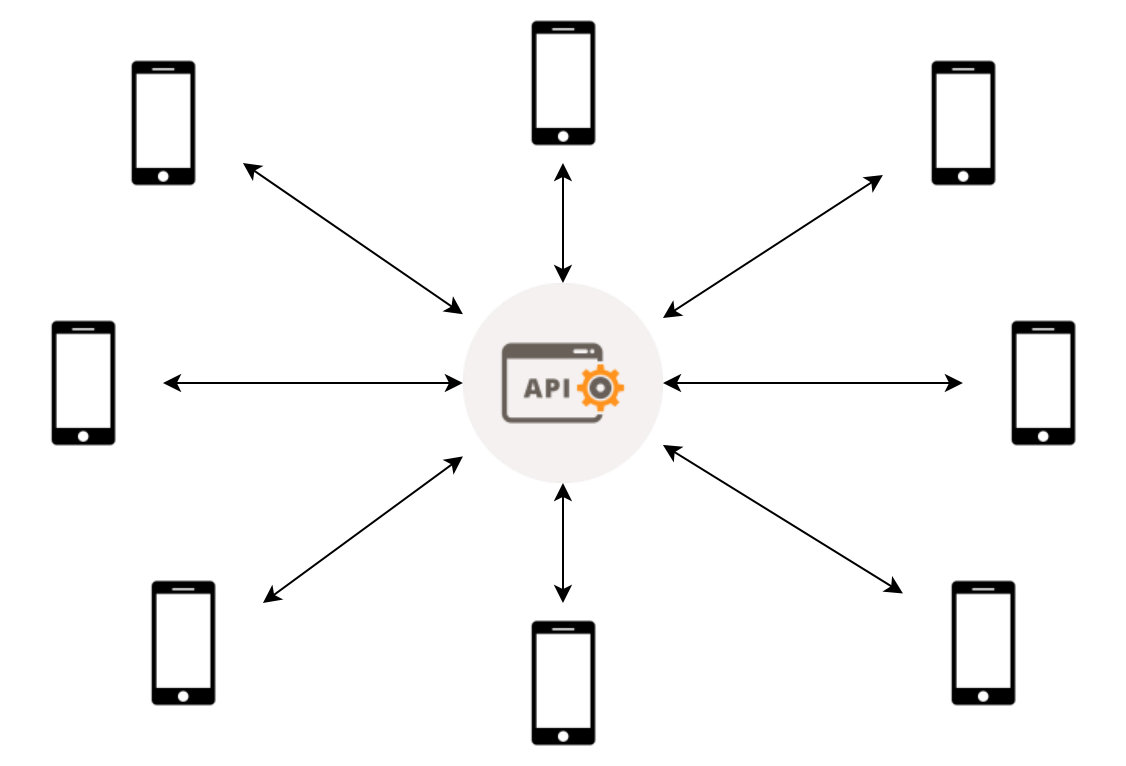
\includegraphics[height=6cm]{../../Resources/Images/capi-ilustration}
    \caption{Ilustrasi CAPI}
    \label{fig:capi-ilustration}
\end{figure}

Tidak terhubungnya suatu \textit{mobile node} dalam sebuah jaringan dapat dikategorikan menjadi 3 (tiga) jenis (Gutwin dkk, 2010) \cite{gutwin_gone_2010}, yaitu:
\begin{itemize}
\item \textit{Delay-based Interruption}, merupakan sebuah gap singkat (\textit{short-term gap}) dalam pengiriman pesan. \textit{Delay} dapat disebabkan oleh berbagai faktor, tetapi porsi terbesar penyebab \textit{delay} adalah \textit{transmission delay}, \textit{contention delay}, dan \textit{queuing delay} ~\cite{zhang_interference-based_2015}.
\item \textit{Network Outage}, merupakan kondisi dimana sebuah \textit{mobile node} terputus dari jaringannya. Kondisi \textit{network outage} dapat disebabkan oleh berbagai faktor, seperti: bencana (kebakaran di \textit{Baltimore Howard Street Tunnel \cite{mcgrattan_numerical_2006}} atau terputusnya \textit{Mediterranean Cable} \cite{zmijewski_mediterranean_2008}), kesalahan konfigurasi (\textit{Pakistani Youtube routing} \cite{hunter_pakistan_2008}), terorisme (misalnya, serangan \textit{World Trade Center} \cite{partridge_internet_2003} atau serangan gelombang elektromagnetik \cite{foster_jr_report_2004}), atau \textit{censorship} (misalnya, respons terhadap kebangkitan masyarakat mesir 2011 \cite{dainotti_analysis_2011})
\item \textit{Explicit Departures}, merupakan kondisi \textit{mobile node} keluar dari jaringan atau keluar dari aplikasi secara eksplisit
\end{itemize}

Brian DeRenzi dkk telah melakukan penelitian tentang cara pengumpulan data berbasis \textit{mobile phone} pada lingkungan yang \textit{highly disconnected} ~\cite{derenzi_reliable_2007} dengan menggunakan \textit{CAM Framework}. \textit{CAM framework}~\cite{parikh_designing_2006} terbukti dapat digunakan dalam pengumpulan data dalam lingkungan yang \textit{disconnected}, dan setelah device kembali ke \textit{connected environment}, data yang terkumpul akan terupload ke server. Akan tetapi \textit{CAM framework} memiliki kelemahan, antara lain : 1) CAM berbasis \textit{fix-length text-based input}, yang membuatnya tidak cocok digunakan untuk pengumpulan data yang mengandung banyak pertanyaan terbuka; 2) Tidak terdapat \textit{conflict resolution}, sehingga masih memungkinkan dua device atau lebih mengeksekusi data yang sama, 3) Tidak terdapat mekanisme pembaharuan aplikasi.

Sementara itu, Takdir dkk telah melalukan penelitian tentang penggunaan pola terdistribusi berbasis SOA ~\cite{takdir_multi-layer_2014}. Pada implementasi pola terdistribusi berbasis SOA, digunakan metode \textit{proxy} baik pada \textit{workflow} (\textit{Web service}) maupun \textit{data-service}. Mekanisme yang digunakan dalam perancangan service pola terdistribusi mencakup 3 (tiga) hal : sinkronisasi, replikasi, dan \textit{routing}. \textit{Composite application} yang dijalankan pada sisi \textit{client} akan melakukan replikasi data maupun \textit{Web service}, kemudian data dan \textit{Web service} tersebut digunakan secara lokal. Sementara itu, untuk menjamin konsistensi data, Takdir dkk mengakomodir mekanisme \textit{sinkronisasi}.

\begin{figure}[h]
    \centering
    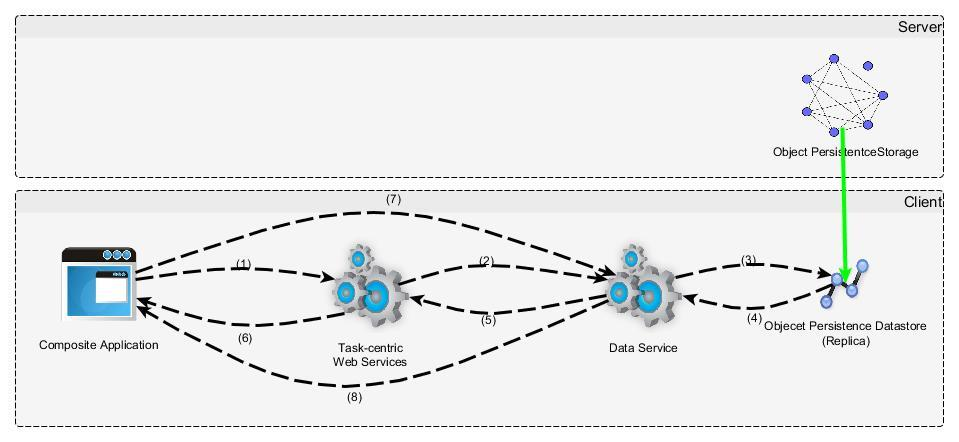
\includegraphics[width=13cm]{../../Resources/Images/takdir-deployment-3a}
    \caption{Skema Usulan, Takdir}
    \label{fig:takdir-soa}
\end{figure}

Berdasarkan hasil pengujian, pola distribusi berbasis SOA usulan Takdir dkk terbukti mampu memberikan hasil yang lebih baik, dengan penggunaan \textit{resource} CPU dan memory yang lebih rendah. Akan tetapi, lingkup perancangan dan pengujian sistem hanya terbatas pada perangkat komputer (\textit{desktop} maupun \textit{laptop}). Pada pola terdistribusi, usulan Takdir dkk, \textit{client} perlu untuk melakukan replikasi data maupun \textit{workflow} yang berupa \textit{Web service} agar dapat berjalan. 

Penelitian ini akan berfokus kepada perancangan metode pengumpulan data berbasis \textit{mobile} yang mendukung \textit{connected environment} maupun \textit{disconnected environment} dengan mengadaptasi mekanisme replikasi, sinkronisasi, dan routing.


\section{Rumusan Masalah}
Berdasarkan uraian latar belakang permasalahan diatas, maka dapat dirumuskan suatu permasalahan penelitian yaitu merancang metode pengumpulan data berbasis \textit{mobile} yang mendukung \textit{connected environment} maupun \textit{disconnected environment}.

\section{Tujuan Penelitian}
Tujuan utama dari penelitian ini adalah menghasilkan rancangan metode pengumpulan data berbasis \textit{mobile} yang mendukung \textit{connected environment} maupun \textit{disconnected environment}. Adapun tujuan khusus penelitian ini adalah :
\begin{itemize}
\item Menghasilkan rancangan mekanisme replikasi data dan \textit{rule} validasi,
\item Menghasilkan rancangan mekanisme sinkronisasi data dan \textit{rule} validasi,
\item Menghasilkan rancangan mekanisme \textit{routing}.
\end{itemize}

\section{Batasan Masalah}
Batasan masalah dalam penelitian ini adalah :

\begin{itemize}
\item Penelitian ini hanya berfokus pada desain dan implementasi sistem pada \textit{mobile device},
\item \textit{Mobile device} yang digunakan dalam ujicoba terbatas hanya \textit{mobile device} dengan sistem operasi \textit{Android}.
\end{itemize}


\section{Batasan Masalah}

Sistematika penulisan tesis ini terdiri atas enam bab dengan perincian sebagai berikut:

\begin{itemize}
\item Pendahuluan\\
Bab ini memuat latar belakang dan motivasi dalam penyusunan penelitian tesis ini serta permasalahan yang ada. Termasuk juga di dalamnya perumusan masalah, tujuan penelitian, manfaat penelitian, batasan masalah, dan keluaran penelitian.

\item Tinjauan Pustaka\\
Bab ini memuat kajian teori dalam penelitian ini. Mencakup berbagai dasar teori yang menjadi landasan dalam penelitian, serta pengetahuan dan informasi tentang penelitian yang pernah dilakukan terkait dengan topik penelitian ini.

\item Metodologi Riset\\
Bab ini memuat tahapan pelaksanaan penlitian mulai dari identifikasi problem sampai urutan penyelesaiannya.

\item Analisis dan Perancangan\\
Bab ini memuat analisis yang dilakukan terhadap masalah yang dihadapi, serta kriteria yang dibutuhkan pada desain yang dirancang. Selain itu, juga diuraikan mengenai rancangan/desain yang dibuat yang juga merupakan solusi yang ditawarkan.

\item Implementasi dan Pengujian\\
Bab ini memuat proses dan hasil implementasi desain yang dirancang. Proses pengujian yang telah dilakukan juga ditampilkan, mulai dari data dan variabel pengukuran yang digunakan, skenario pengujian, hingga hasil pengujian.

\item Kesimpulan dan Saran\\
Bab ini memuat kesimpulan yang diperoleh dari penelitian ini, serta saran untuk pihak terkait dan untuk penelitian selanjutnya yang berkaitan dengan topik penelitian ini.
\end{itemize}

